%====================================================%
% SEZIONE 1: Tubo a U
%====================================================%
\begin{question}[ID=1.1, subtitle={Tubo a U con acqua e olio}, tags={fluidi, pressione, tubo a U}, difficulty=facile]
Un tubo a U contiene acqua ($\rho = 1000\ \mathrm{kg/m^3}$) e olio ($\rho = 800\ \mathrm{kg/m^3}$). L'olio viene versato in uno dei due rami e forma una colonna alta 20 cm. Di quanto si abbassa il livello dell'acqua nello stesso ramo rispetto all'altro?
\begin{solution}
All'equilibrio le pressioni al fondo devono essere uguali. Sia $\Delta h$ l'abbassamento dell'acqua:
\[
\rho_{olio}\,g\,h_{olio} = \rho_{acqua}\,g\,\Delta h
\;\Rightarrow\;
\Delta h = \frac{800 \cdot 0{,}20}{1000} = 0{,}16\ \mathrm{m} = \mathbf{16\ cm}.
\]
\end{solution}
\end{question}

%-----------------------------------------------%

\begin{question}[ID=1.2, subtitle={Tubo a U con acqua e mercurio}, tags={fluidi, pressione, tubo a U}, difficulty=facile]
In un tubo a U aperto, un ramo contiene acqua e l'altro mercurio ($\rho = 13600\ \mathrm{kg/m^3}$). Se la differenza di altezza tra i due livelli del mercurio è 4 cm, qual è la differenza di altezza della colonna d'acqua necessaria per bilanciare la pressione?
\begin{solution}
All'equilibrio le due colonne devono esercitare la stessa pressione idrostatica alla base; poiché $p = \rho g h$, uguagliamo i prodotti $\rho\,h$ dei due liquidi e ricaviamo l'altezza della colonna d'acqua:
\[
\rho_{Hg}\,g\,h_{Hg} = \rho_{acqua}\,g\,h_{acqua}
\;\Rightarrow\;
h_{acqua} = \frac{13600 \cdot 0{,}04}{1000} = 0{,}544\ \mathrm{m} \approx \mathbf{54{,}4\ cm}.
\]
Essendo il mercurio molto più denso, basta una sua colonna sottile per bilanciare una colonna d'acqua oltre dieci volte più alta.
\end{solution}
\end{question}

%-----------------------------------------------%

\begin{question}[ID=1.3, subtitle={Tubo a U con acqua e glicerina}, tags={fluidi, pressione, tubo a U}, difficulty=facile]
\begin{wrapfigure}{r}{0.25\textwidth}
    \centering
    \vspace{-40pt}
    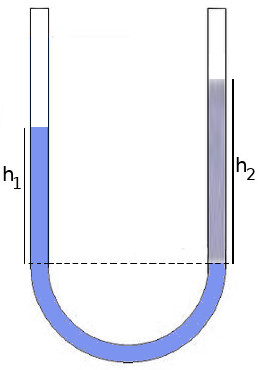
\includegraphics[width=0.15\textwidth]{images/tubo_U}
\end{wrapfigure}

Un tubo a U aperto da entrambe le estremità contiene acqua e glicerina ($\rho_{glicerina} = 1260\ \mathrm{kg/m^3}$). La colonna d'acqua misura 30 cm.
\begin{enumerate}
    \item Calcola l'altezza della colonna di glicerina necessaria per bilanciare la pressione.
\end{enumerate}
\begin{solution}
All'equilibrio le pressioni idrostatiche alla base dei due rami sono uguali, $\rho_{acqua}\,h_{acqua} = \rho_{glicerina}\,h_{glicerina}$. Essendo la glicerina più densa dell'acqua, la sua colonna sarà più bassa:
\[
h_{glicerina} = \frac{\rho_{acqua}}{\rho_{glicerina}}\,h_{acqua} = \frac{1000}{1260} \cdot 0{,}30 \approx 0{,}238\ \mathrm{m} \approx \mathbf{23{,}8\ cm}.
\]
\end{solution}
\end{question}

%-----------------------------------------------%

\begin{question}[ID=1.4, subtitle={Tubo a U con mercurio e colonna d'acqua}, tags={fluidi, pressione, tubo a U}, difficulty=media]
In un tubo a U con mercurio, nell'estremità aperta viene aggiunta acqua fino a formare una colonna alta 60 cm. Pressione atmosferica $p_0 = 1{,}01\times10^5\ \mathrm{Pa}$, $\rho_{Hg} = 13600\ \mathrm{kg/m^3}$. Determina la differenza di livello del mercurio tra i due rami.
\begin{solution}
La colonna d'acqua esercita una pressione $\Delta p = \rho_{acqua}\,g\,h = 1000 \cdot 9{,}81 \cdot 0{,}60 = 5886\ \mathrm{Pa}$.
La differenza di livello del mercurio:
\[
\Delta h_{Hg} = \frac{\Delta p}{\rho_{Hg}\,g} = \frac{5886}{13600 \cdot 9{,}81} \approx 0{,}044\ \mathrm{m} \approx \mathbf{4{,}4\ cm}.
\]
\end{solution}
\end{question}

%====================================================%
% SEZIONE 2: Principio di Pascal — martinetto idraulico
%====================================================%
\begin{question}[ID=2.1, subtitle={Forza sul pistone piccolo del martinetto}, tags={fluidi, Pascal, martinetto}, difficulty=facile]
Un martinetto idraulico ha due pistoni: piccolo con area $A_1 = 5\ \mathrm{cm^2}$ e grande con area $A_2 = 100\ \mathrm{cm^2}$. Quale forza deve essere applicata sul pistone piccolo per sollevare un carico di 2000 N?
\begin{solution}
Per il principio di Pascal $p_1 = p_2$:
\[
\frac{F_1}{A_1} = \frac{F_2}{A_2}
\;\Rightarrow\;
F_1 = F_2\,\frac{A_1}{A_2} = 2000 \cdot \frac{5}{100} = \mathbf{100\ \mathrm{N}}.
\]
\end{solution}
\end{question}

%-----------------------------------------------%

\begin{question}[ID=2.2, subtitle={Forza amplificata dal sistema idraulico}, tags={fluidi, Pascal, martinetto}, difficulty=facile]
In un sistema idraulico, una forza di 150 N viene applicata su un pistone con area $10\ \mathrm{cm^2}$. Qual è la forza risultante su un pistone con area $50\ \mathrm{cm^2}$?
\begin{solution}
Per il principio di Pascal la pressione si trasmette inalterata nel fluido ($p_1 = p_2$), quindi le forze sui due pistoni stanno tra loro come le rispettive aree:
\[
F_2 = F_1\,\frac{A_2}{A_1} = 150 \cdot \frac{50}{10} = \mathbf{750\ \mathrm{N}}.
\]
\end{solution}
\end{question}

%-----------------------------------------------%

\begin{question}[ID=2.3, subtitle={Martinetto con pistoni di diametro 2 cm e 10 cm}, tags={fluidi, Pascal, martinetto}, difficulty=facile]
Un martinetto ha pistone piccolo con diametro $2\ \mathrm{cm}$ e grande con diametro $10\ \mathrm{cm}$. Se si applica 80 N sul pistone piccolo, qual è la forza sul grande?
\begin{solution}
Calcoliamo le aree dei due pistoni circolari ($A = \pi r^2$):
\[
A_1 = \pi\,(0{,}01)^2 = 3{,}14\times10^{-4}\ \mathrm{m^2}, \qquad A_2 = \pi\,(0{,}05)^2 = 7{,}85\times10^{-3}\ \mathrm{m^2}.
\]
Per il principio di Pascal la forza è amplificata in proporzione al rapporto delle aree, cioè al quadrato del rapporto dei diametri:
\[
F_2 = F_1\,\frac{A_2}{A_1} = 80\cdot\frac{(0{,}05)^2}{(0{,}01)^2} = 80\cdot 25 = \mathbf{2000\ \mathrm{N}}.
\]
\end{solution}
\end{question}

%-----------------------------------------------%

\begin{question}[ID=2.4, subtitle={Pressione per sostenere un'automobile sul martinetto}, tags={fluidi, Pascal, martinetto}, difficulty=facile]
Un martinetto ha pistone grande con area $150\ \mathrm{cm^2}$ che solleva un'automobile di massa 1200 kg. Quale pressione nel liquido mantiene l'equilibrio?
\begin{solution}
Il liquido deve esercitare sul pistone grande una pressione tale che la forza risultante $p\,A$ equilibri il peso dell'automobile. La pressione è quindi il peso diviso l'area del pistone:
\[
p = \frac{F}{A} = \frac{1200 \cdot 9{,}81}{150\times10^{-4}} = \frac{11772}{0{,}015} \approx \mathbf{7{,}85\times10^{5}\ \mathrm{Pa}}.
\]
\end{solution}
\end{question}

%-----------------------------------------------%

\begin{question}[ID=2.5, subtitle={Area del pistone maggiore dato il rapporto di forze}, tags={fluidi, Pascal, martinetto}, difficulty=facile]
Un operaio applica 60 N su un pistone con area $0{,}002\ \mathrm{m^2}$. La forza risultante sull'altro pistone è 1800 N. Qual è l'area del pistone maggiore?
\begin{solution}
Per il principio di Pascal le aree dei due pistoni stanno tra loro come le forze ($A_2/A_1 = F_2/F_1$). Ricaviamo quindi l'area del pistone maggiore:
\[
A_2 = A_1\,\frac{F_2}{F_1} = 0{,}002\cdot\frac{1800}{60} = \mathbf{0{,}06\ \mathrm{m^2}}.
\]
\end{solution}
\end{question}

%====================================================%
% SEZIONE 3: Principio di Archimede
%====================================================%
\begin{question}[ID=3.1, subtitle={Sfera cava in acciaio immersa in acqua}, tags={fluidi, Archimede, galleggiamento}, difficulty=media]
Una sfera cava in acciaio ha raggio esterno $R = 0{,}10\ \mathrm{m}$ e spessore $2\ \mathrm{mm}$. $\rho_{acciaio} = 7850\ \mathrm{kg/m^3}$.
\begin{enumerate}
    \item Qual è la massa della sfera?
    \item Qual è la spinta di Archimede?
    \item Galleggia o affonda?
\end{enumerate}
\begin{solution}
\begin{enumerate}
    \item $V_{acciaio} \approx 4\pi R^2\,s = 4\pi\,(0{,}10)^2\,0{,}002 \approx 2{,}51\times10^{-4}\ \mathrm{m^3}$;\quad $m = \rho\,V \approx 1{,}97\ \mathrm{kg}$.
    \item $F_A = \rho_{acqua}\,g\,V_{sfera} = 1000\cdot9{,}81\cdot\tfrac{4}{3}\pi(0{,}10)^3 \approx 41{,}1\ \mathrm{N}$;\quad peso $= mg \approx 19{,}3\ \mathrm{N}$.
    \item Poiché $F_A > P$, la sfera \textbf{galleggia}.
\end{enumerate}
\end{solution}
\end{question}

%-----------------------------------------------%

\begin{question}[ID=3.2, subtitle={Corpo che galleggia con metà volume immerso}, tags={fluidi, Archimede, galleggiamento}, difficulty=facile]
Un corpo di volume $0{,}002\ \mathrm{m^3}$ galleggia con metà del volume immerso in acqua.
\begin{enumerate}
    \item Qual è la spinta di Archimede?
    \item Qual è la massa del corpo?
    \item Qual è la sua densità?
\end{enumerate}
\begin{solution}
\begin{enumerate}
    \item La spinta di Archimede è il peso del fluido spostato, cioè $\rho_{acqua}\,g$ moltiplicato per il volume immerso (metà del volume totale, $0{,}001\ \mathrm{m^3}$):
    \[
    F_A = \rho_{acqua}\,g\,V_{immerso} = 1000\cdot 9{,}81\cdot 0{,}001 = \mathbf{9{,}81\ \mathrm{N}}.
    \]
    \item Il corpo galleggia in equilibrio, quindi la spinta bilancia il peso ($F_A = mg$):
    \[
    m = \frac{F_A}{g} = \frac{9{,}81}{9{,}81} = \mathbf{1{,}00\ \mathrm{kg}}.
    \]
    \item La densità è massa su volume (totale):
    \[
    \rho = \frac{m}{V} = \frac{1{,}00}{0{,}002} = \mathbf{500\ \mathrm{kg/m^3}},
    \]
    cioè metà di quella dell'acqua, coerente col fatto che galleggia per metà immerso.
\end{enumerate}
\end{solution}
\end{question}

%-----------------------------------------------%

\begin{question}[ID=3.3, subtitle={Pallina di plastica in acqua e in olio}, tags={fluidi, Archimede, galleggiamento}, difficulty=media]
Una pallina di plastica con massa $0{,}03\ \mathrm{kg}$ e volume $5\times10^{-5}\ \mathrm{m^3}$ viene immersa:
\begin{enumerate}
    \item in acqua ($\rho = 1000\ \mathrm{kg/m^3}$)
    \item in olio ($\rho = 800\ \mathrm{kg/m^3}$)
\end{enumerate}
In entrambi i casi calcolare la spinta di Archimede e se la pallina galleggia o affonda.
\begin{solution}
Peso della pallina: $P = 0{,}03 \cdot 9{,}81 = 0{,}294\ \mathrm{N}$.
\begin{enumerate}
    \item $F_{A,acqua} = 1000\cdot9{,}81\cdot5\times10^{-5} = 0{,}491\ \mathrm{N} > P$ → \textbf{galleggia}.
    \item $F_{A,olio} = 800\cdot9{,}81\cdot5\times10^{-5} = 0{,}392\ \mathrm{N} > P$ → \textbf{galleggia}.
\end{enumerate}
\end{solution}
\end{question}

%====================================================%
% SEZIONE 4: Problemi misti su pressione e Archimede
%====================================================%
\begin{question}[ID=4.1, subtitle={Pressione e forza su martinetto con aree 12 e 96 cm²}, tags={fluidi, Pascal, martinetto}, difficulty=facile]
Un martinetto ha pistone piccolo $A_1 = 12\ \mathrm{cm^2}$ e grande $A_2 = 96\ \mathrm{cm^2}$. Sul pistone piccolo si applica 30 N.
\begin{enumerate}
    \item Qual è la pressione esercitata sul fluido?
    \item Qual è la forza risultante sul pistone grande?
\end{enumerate}
\begin{solution}
\begin{enumerate}
    \item La pressione trasmessa al fluido è la forza applicata diviso l'area del pistone piccolo:
    \[
    p = \frac{F_1}{A_1} = \frac{30}{12\times10^{-4}} = 2500\ \mathrm{Pa}.
    \]
    \item Per il principio di Pascal questa stessa pressione agisce sul pistone grande, generando una forza pari a $p\,A_2$:
    \[
    F_2 = p\cdot A_2 = 2500\cdot 96\times10^{-4} = \mathbf{240\ \mathrm{N}}.
    \]
\end{enumerate}
\end{solution}
\end{question}

%-----------------------------------------------%

\begin{question}[ID=4.2, subtitle={Pressione trasmessa da forza su pistone circolare}, tags={fluidi, Pascal}, difficulty=facile]
Una forza di 50 N è applicata su un pistone con diametro $2\ \mathrm{cm}$. Qual è la pressione trasmessa al fluido?
\begin{solution}
La pressione è la forza diviso l'area del pistone. Calcoliamo prima l'area del pistone circolare (raggio $1\ \mathrm{cm}$):
\[
A = \pi\,(0{,}01)^2 = 3{,}14\times10^{-4}\ \mathrm{m^2}.
\]
Quindi la pressione trasmessa al fluido è
\[
p = \frac{F}{A} = \frac{50}{3{,}14\times10^{-4}} \approx \mathbf{1{,}59\times10^{5}\ \mathrm{Pa}}.
\]
\end{solution}
\end{question}

%-----------------------------------------------%

\begin{question}[ID=4.3, subtitle={Martinetto che solleva un'auto da 2 tonnellate}, tags={fluidi, Pascal, martinetto}, difficulty=media]
Un martinetto solleva un'auto di massa $2\ \mathrm{t}$. L'area della piattaforma è $15\ \mathrm{m^2}$, la forza sul pistone piccolo è $300\ \mathrm{N}$.
\begin{enumerate}
    \item Calcola la pressione esercitata dall'auto sulla piattaforma.
    \item Calcola l'area del pistone piccolo.
\end{enumerate}
\begin{solution}
\begin{enumerate}
    \item La pressione esercitata dall'auto sulla piattaforma è il suo peso diviso l'area della piattaforma:
    \[
    p = \frac{F}{A} = \frac{2000\cdot 9{,}81}{15} \approx \mathbf{1308\ \mathrm{Pa}}.
    \]
    \item Per il principio di Pascal questa pressione è la stessa nel pistone piccolo; l'area si ottiene quindi dividendo la forza applicata per la pressione:
    \[
    A_{piccolo} = \frac{F_{piccolo}}{p} = \frac{300}{1308} \approx \mathbf{0{,}229\ \mathrm{m^2}}.
    \]
\end{enumerate}
\end{solution}
\end{question}

%-----------------------------------------------%

\begin{question}[ID=4.4, subtitle={Pressione nel martinetto per sollevare 1000 N}, tags={fluidi, Pascal}, difficulty=facile]
Un carico di 1000 N viene sollevato da un martinetto con pistone grande di diametro 20 cm. Qual è la pressione nel liquido?
\begin{solution}
Il liquido sostiene il carico esercitando sul pistone una pressione pari alla forza diviso l'area. L'area del pistone (raggio $10\ \mathrm{cm}$) è
\[
A = \pi\,(0{,}10)^2 = 3{,}14\times10^{-2}\ \mathrm{m^2},
\]
da cui la pressione nel liquido:
\[
p = \frac{F}{A} = \frac{1000}{3{,}14\times10^{-2}} \approx \mathbf{3{,}18\times10^{4}\ \mathrm{Pa}}.
\]
\end{solution}
\end{question}

%-----------------------------------------------%

\begin{question}[ID=4.5, subtitle={Martinetto idraulico: forza, rapporto aree e moltiplicazione}, tags={fluidi, Pascal, martinetto}, difficulty=media]
Un martinetto ha pistone piccolo $A_1 = 0{,}0015\ \mathrm{m^2}$ e grande $A_2 = 0{,}045\ \mathrm{m^2}$.
\begin{enumerate}
    \item Che forza è necessaria sul pistone piccolo per sollevare 1350 N?
    \item Il sistema moltiplica o riduce la forza?
    \item Qual è il rapporto tra le aree?
\end{enumerate}
\begin{solution}
\begin{enumerate}
    \item $F_1 = 1350\cdot(0{,}0015/0{,}045) = 1350/30 = 45\ \mathrm{N}$.
    \item Il sistema \textbf{moltiplica} la forza (applichi 45 N e ottieni 1350 N).
    \item $A_2/A_1 = 0{,}045/0{,}0015 = 30$.
\end{enumerate}
\end{solution}
\end{question}

%====================================================%
% SEZIONE 5: Pressione idrostatica
%====================================================%
\begin{question}[ID=5.1, subtitle={Sottomarino a 450 m di profondità}, tags={fluidi, pressione idrostatica}, difficulty=media]
Un sottomarino si immerge alla profondità di $450\ \mathrm{m}$. $\rho_{acqua\,marina} = 1033\ \mathrm{kg/m^3}$.
\begin{enumerate}
    \item Calcola la pressione agente sul sottomarino (inclusa quella atmosferica).
    \item Che forza viene esercitata sul portellone di superficie $S = 0{,}50\ \mathrm{m^2}$?
    \item Calcola la massima profondità se il portellone ha resistenza massima $15{,}2\times10^6\ \mathrm{N}$.
\end{enumerate}
\begin{solution}
\begin{enumerate}
    \item La pressione totale è la somma di quella atmosferica in superficie e di quella idrostatica della colonna d'acqua sovrastante ($\rho g h$):
    \[
    p = p_0 + \rho g h = 1{,}01\times10^5 + 1033\cdot 9{,}81\cdot 450 \approx \mathbf{4{,}66\times10^6\ \mathrm{Pa}}.
    \]
    \item La forza sul portellone è la pressione moltiplicata per la sua superficie:
    \[
    F = p\cdot S = 4{,}66\times10^6\cdot 0{,}50 \approx \mathbf{2{,}33\times10^6\ \mathrm{N}}.
    \]
    \item La profondità massima si ottiene imponendo che la forza sul portellone raggiunga il valore di rottura $F_{max}$; invertendo le relazioni precedenti rispetto a $h$:
    \[
    h_{max} = \frac{F_{max}/S - p_0}{\rho g} = \frac{15{,}2\times10^6/0{,}50 - 1{,}01\times10^5}{1033\cdot 9{,}81} \approx \mathbf{2990\ \mathrm{m}}.
    \]
\end{enumerate}
\end{solution}
\end{question}

%-----------------------------------------------%

\begin{question}[ID=6.1, subtitle={Raggio di una sfera in equilibrio sotto il pelo dell'acqua}, tags={fluidi, Archimede, galleggiamento}, difficulty=media]
Calcola il raggio di una sfera piena di massa $m = 700\ \mathrm{g}$ in equilibrio che galleggia sotto il pelo dell'acqua dolce.
\begin{solution}
Per galleggiare completamente immersa: $\rho_{sfera} = \rho_{acqua}$. La massa della sfera immersa eguaglia la massa d'acqua spostata:
\[
m = \rho_{acqua}\,\tfrac{4}{3}\pi R^3
\;\Rightarrow\;
R = \left(\frac{3m}{4\pi\rho_{acqua}}\right)^{1/3} = \left(\frac{3\cdot0{,}700}{4\pi\cdot1000}\right)^{1/3} \approx 0{,}0549\ \mathrm{m} \approx \mathbf{5{,}5\ cm}.
\]
\end{solution}
\end{question}

%-----------------------------------------------%

\begin{question}[ID=6.2, subtitle={Corona di Gerone: oro o argento?}, tags={fluidi, Archimede, densità}, difficulty=difficile]
La corona di Gerone ha massa $0{,}802\ \mathrm{kg}$ e peso in acqua $7{,}19\ \mathrm{N}$.
\begin{enumerate}
    \item Determina se la corona è composta interamente d'oro ($\rho_{Au} = 19300\ \mathrm{kg/m^3}$, $\rho_{Ag} = 10500\ \mathrm{kg/m^3}$).
    \item In caso contrario determina il volume di oro e di argento.
\end{enumerate}
\begin{solution}
Peso in aria: $P = 0{,}802\cdot9{,}81 = 7{,}867\ \mathrm{N}$. Spinta di Archimede: $F_A = 7{,}867 - 7{,}19 = 0{,}677\ \mathrm{N}$.
Volume totale: $V_{tot} = F_A/(\rho_{acqua}\,g) = 0{,}677/9810 = 6{,}90\times10^{-5}\ \mathrm{m^3}$.
Se fosse d'oro puro: $V_{Au} = m/\rho_{Au} = 0{,}802/19300 = 4{,}16\times10^{-5}\ \mathrm{m^3} \neq V_{tot}$ → \textbf{non è oro puro}.

Sistema: $V_{Au} + V_{Ag} = 6{,}90\times10^{-5}$ e $\rho_{Au}V_{Au} + \rho_{Ag}V_{Ag} = 0{,}802\ \mathrm{kg}$.
Risolvendo: $V_{Au} \approx 3{,}02\times10^{-5}\ \mathrm{m^3}$;\quad $V_{Ag} \approx 3{,}88\times10^{-5}\ \mathrm{m^3}$.
\end{solution}
\end{question}

%-----------------------------------------------%

\begin{question}[ID=7.1, subtitle={Equazione di Bernoulli in tubo che si restringe e sale}, tags={fluidi, Bernoulli, continuità}, difficulty=difficile]
\begin{wrapfigure}{r}{0.25\textwidth}
    \centering
    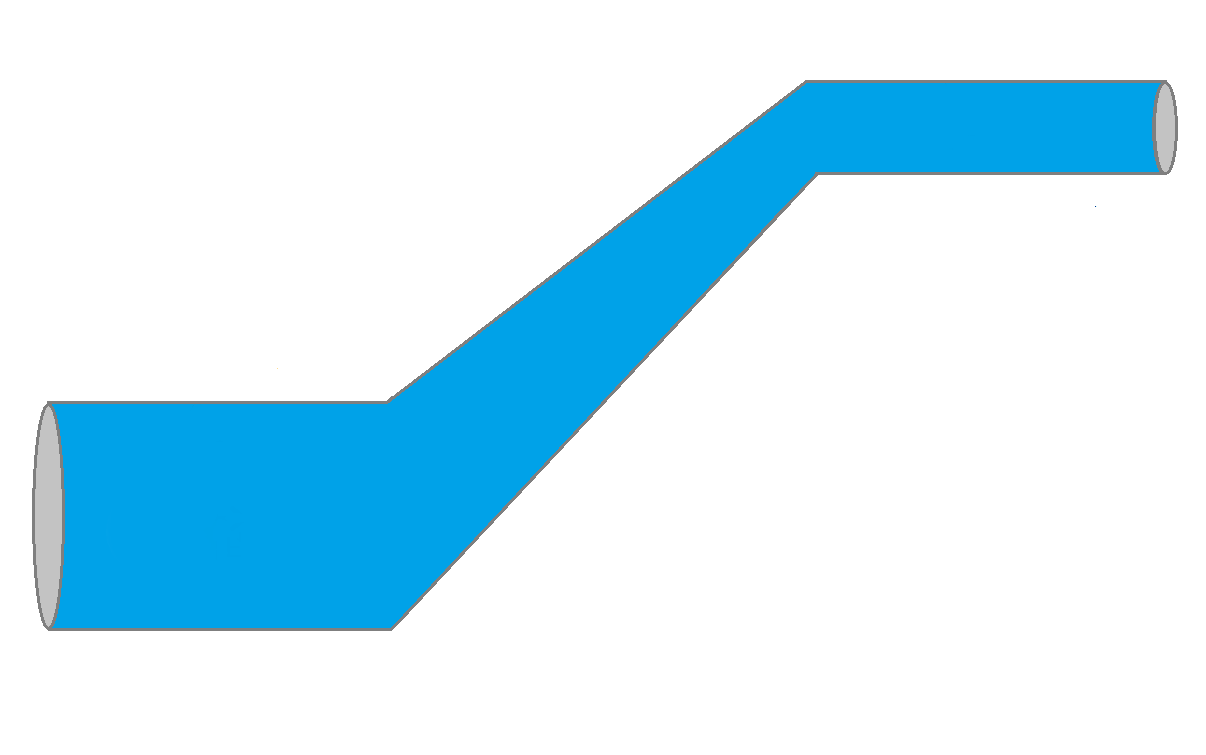
\includegraphics[width=0.25\textwidth]{images/Tubo_flusso_bernoulli}
\end{wrapfigure}
Un impianto idrico ha una tubazione cilindrica con diametro iniziale $10\ \mathrm{cm}$ che si innalza di $3\ \mathrm{m}$ riducendosi a diametro $4\ \mathrm{cm}$. Nella parte bassa l'acqua scorre a $v_1 = 5\ \mathrm{m/s}$.
\begin{enumerate}
    \item Calcola la velocità nella sezione più stretta.
    \item Calcola la differenza di pressione tra i due tratti.
\end{enumerate}
\begin{solution}
\begin{enumerate}
    \item Equazione di continuità: $A_1 v_1 = A_2 v_2$:
    \[
    v_2 = v_1\,\frac{A_1}{A_2} = 5\cdot\frac{(0{,}05)^2}{(0{,}02)^2} = 5\cdot\frac{25}{4} = 31{,}25\ \mathrm{m/s}.
    \]
    \item Bernoulli ($\rho = 1000\ \mathrm{kg/m^3}$, $\Delta h = 3\ \mathrm{m}$):
    \[
    \Delta p = p_1 - p_2 = \tfrac{1}{2}\rho(v_2^2 - v_1^2) + \rho g \Delta h
    = \tfrac{1}{2}\cdot1000\cdot(976{,}6 - 25) + 1000\cdot9{,}81\cdot3
    \approx 505\ 000\ \mathrm{Pa}.
    \]
\end{enumerate}
\end{solution}
\end{question}

\begin{question}[ID=7.2, subtitle={Corona di Gerone — FAC: composizione con densità}, tags={fluidi, Archimede, densità}, difficulty=difficile]
\textbf{FAC)} La corona di Gerone ha massa $0{,}802\ \mathrm{kg}$ e peso apparente in acqua $7{,}19\ \mathrm{N}$. Utilizzando $\rho_{Au} = 19300\ \mathrm{kg/m^3}$ e $\rho_{Ag} = 10500\ \mathrm{kg/m^3}$:
\begin{enumerate}
    \item Determina se la corona è composta interamente d'oro.
    \item In caso contrario determina il volume di oro e di argento.
\end{enumerate}
\begin{solution}
Vedi esercizio 6.2 per la soluzione completa.
\end{solution}
\end{question}
